\chapter{The Gauss circle problem and its generalizations}\label{gauss-circle-chapter}

\unintegrated

For any fixed integer $k \ge 2$ and unbounded $R$, consider the problem of estimating the number of integer lattice points contained in $B_k(R)$, a $k$-dimensional ball of radius $R$:
\[
S_k(R) := \# \mathbb{Z}^k \cap B_k(R) = \# \{x \in \mathbb{Z}^k: |x| \le R\}.
\]
Equivalently, $S_k(R)$ may be written as the partial sum 
\[
S_k(R) = \sum_{n \le R^{2}}r_k(n)
\]
where $r_k(n)$ counts the number of integer solutions to the equation $x_1^2 + \cdots + x_k^2 = n$.

By considering the volume of a $k$-dimensional ball of radius $R$, one has the asymptotic
\[
S_k(R) \sim \operatorname{Vol}(B_k(R)) = \frac{\pi^{k/2}}{\Gamma(k/2 + 1)}R^k.
\]
The generalized Gauss circle problem concerns estimating the error term in this approximation. 

\begin{definition}
For fixed integer $k \ge 2$, define $\theta^{\operatorname{Gauss}}_{k}$ as the least (fixed) exponent for which
\[
S_k(R) - \operatorname{Vol}(B_k(R)) \ll R^{\theta^{\operatorname{Gauss}}_{k} + o(1)}.
\]
\end{definition}

\Cref{fig:gauss_circle_2} and \Cref{fig:gauss_circle_3} plots the magnitude of this error term for $k = 2$ and $k = 3$ respectively (for $0 < R \le 1000$).

\begin{figure}
    \centering
    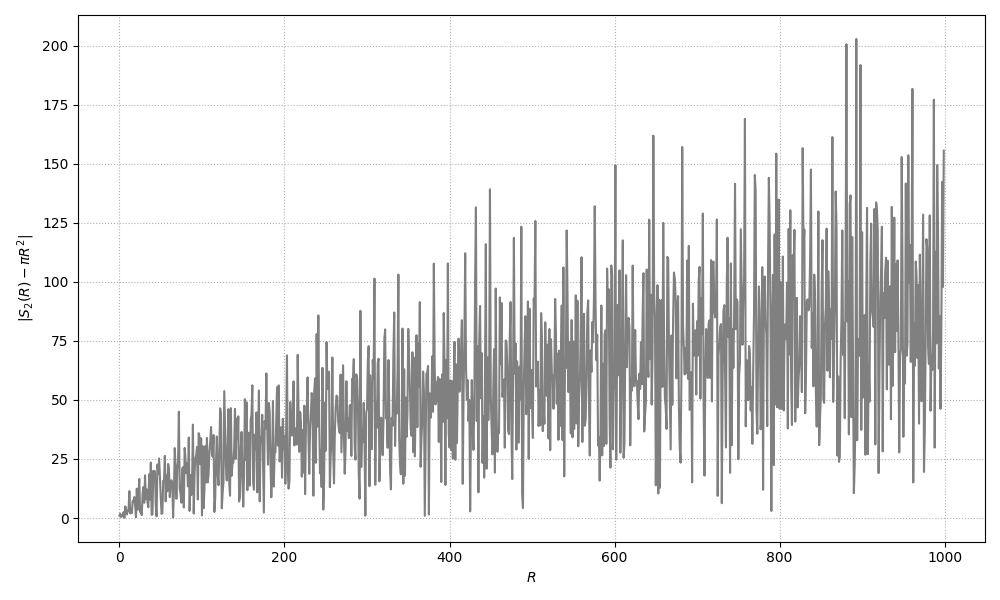
\includegraphics[width=0.5\linewidth]{chapter/gauss_circle_error_2.png}
    \caption{$|S_k(R) - \operatorname{Vol}(B_k(R))|$ for $k = 2$ and $0 < R \le 1000$}
    \label{fig:gauss_circle_2}
\end{figure}

\begin{figure}
    \centering
    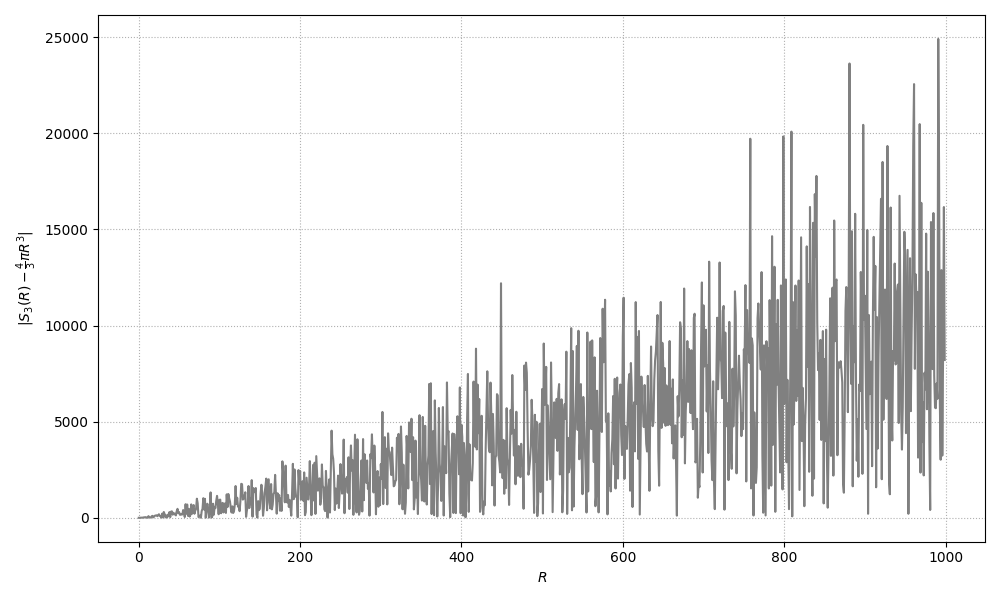
\includegraphics[width=0.5\linewidth]{chapter/gauss_circle_error_3.png}
    \caption{$|S_k(R) - \operatorname{Vol}(B_k(R))|$ for $k = 3$ and $0 < R \le 1000$}
    \label{fig:gauss_circle_3}
\end{figure}


It is conjectured that 

\begin{conjecture}\label{gauss-circle-conj}
One has 
\[
\theta^{\operatorname{Gauss}}_{k} = \begin{cases}
1/2,& k = 2,\\
k - 2,& k \ge 3.
\end{cases}
\]
\end{conjecture}


\section{Known upper and lower bounds}

\Cref{gauss-circle-conj} is known to hold for $k \ge 4$, i.e.

\begin{theorem}
For integer $k \ge 4$, one has $\theta^{\operatorname{Gauss}}_{k} = k - 2$.
\end{theorem}

The remaining open cases are $k = 2, 3$. For such cases the following lower-bounds on $\theta^{\operatorname{Gauss}}_{k}$ are known:

\begin{theorem}\label{gauss-circle-lower-23}
One has $\theta^{\operatorname{Gauss}}_{2} \ge 1/2$ and $\theta^{\operatorname{Gauss}}_{3} \ge 1$.
\end{theorem}

In light of \Cref{gauss-circle-conj} and \Cref{gauss-circle-lower-23}, in the rest of this section we shall focus on upper bounds on $\theta^{\operatorname{Gauss}}_{k}$ for $k = 2, 3$.

The case $k = 2$ is known classically as Gauss's circle problem. The current sharpest known bound on $\theta_2^{\operatorname{Gauss}}$ is
\begin{theorem}[Li--Yang (2023) \cite{li_yang_gauss_2024}] 
One has $\theta_2^{\operatorname{Gauss}} \le 2\alpha$, where $\alpha = 0.31448\ldots$ is the solution to the equation
\[
\frac{8}{25}\alpha - \frac{(\sqrt{2(1+14\alpha)} - 5\sqrt{-1+8\alpha})^2}{200} + \frac{51}{200} = \alpha
\]
on the interval $[0.3, 0.35]$.
\end{theorem}

\begin{remark}
The value of $\alpha$ is the same as that appearing in \Cref{divisor-2-bound}. Historically, methods used to make progress in the $\alpha_2$ exponent in the Dirichlet divisor problem have led to corresponding improvements in $\theta_2^{\operatorname{Gauss}}$ (and vice versa). This may be unsurprising given that both problems reduce to counting the number of lattice points contained in a curved region with a smooth boundary (with the region being the hyperbola $\{(m,n) \in [0, \infty)^2: mn \le x \}$ in the case of the Dirichlet divisor problem).
\end{remark}

The historical progression of upper bounds on $\theta_2^{\operatorname{Gauss}}$ is recorded in \Cref{gauss-circle-table-2} and \Cref{fig:gauss_circle_historical}.


\begin{table}[ht]
    \def\arraystretch{1.2}
    \centering
    \caption{Historical upper bounds on $\theta_2^{\operatorname{Gauss}}$}
    \begin{tabular}{|c|c|}
    \hline
    Reference & Bound on $\theta_2^{\operatorname{Gauss}}$\\
    \hline
    Gauss (1834) & $1$\\
    \hline
    Sierpi\'nski (1906) \cite{sierpinski_pewnem_1906} & $2/3 = 0.6666\ldots$\\
    \hline
    van der Corput (1923) \cite{van_der_corput_neue_1923} & $2/3 - \delta$ for some $\delta > 0$\\
    \hline
    Littlewood--Walfisz (1924) \cite{littlewood_lattice_1924} & $37/56 = 0.6607\ldots$\\
    \hline
    Walfisz (1927) \cite{walfisz_teilerprobleme_1927} & $163/247 = 0.6599\ldots$\\
    \hline
    Nieland (1928) \cite{nieland_zum_1928} & $27/41 = 0.6585\ldots$\\
    \hline
    Titchmarsh (1935) \cite{titchmarsh_lattice_points_1935} & $15/23 = 0.6521\ldots$\\
    \hline
    Hua (1942) \cite{hua_lattice_points_1942} & $13/20 = 0.65$\\
    \hline
    Iwaniec--Mozzochi (1988) \cite{iwaniec_divisor_1988} & $7/11 = 0.6363\ldots$ \\
    \hline
    Huxley (1993) \cite{huxley_lattice_1993} & $46/73 = 0.6301\ldots$\\
    \hline
    Huxley (2003) \cite{huxley_exponential_2003} & $131/208 = 0.6298\ldots$\\
    \hline
    Li--Yang (2023) \cite{li_yang_gauss_2024} & $2\alpha* = 0.6289\ldots$\\
    \hline 
    \end{tabular}
\label{gauss-circle-table-2}
\end{table}

\begin{figure}
    \centering
    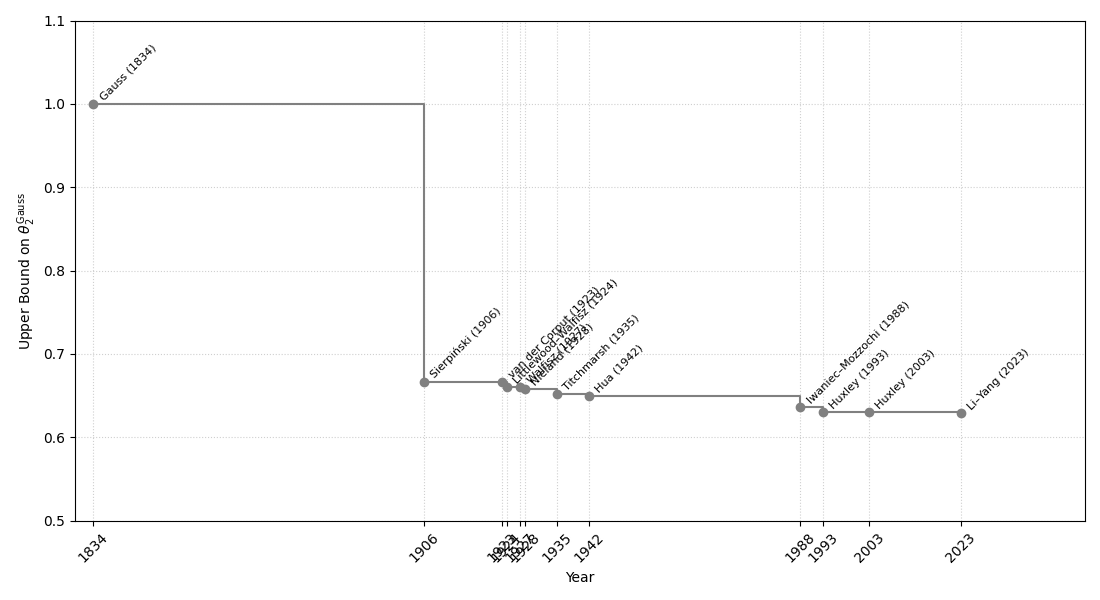
\includegraphics[width=0.5\linewidth]{chapter/gauss_circle_historical_bounds.png}
    \caption{Historical upper bounds on $\theta_2^{\rm Gauss}$}
    \label{fig:gauss_circle_historical}
\end{figure}